Now that we have presented the coordination facts for LM,
Fig.~\ref{code:shortest_path_program_coord} shows an example of their usage by
extending the SSSP program presented before. The coordinated version of the SSSP
program uses a global program directive to order priorities in ascending order
(line~\ref{line:coord:sssp_asc}) and the coordination fact \code{set-priority}
(line~\ref{line:coord:sssp_set}). The proof of correctness for this program is
presented in Appendix~\ref{appendix:proofs:sssp}.

\begin{figure}[ht]
\begin{Verbatim}[numbers=left,commandchars=\\\{\},fontsize=\codesize]
type edge(node, node, int).\hfill// Predicate declaration
type linear shortest(node, int, list int).
type linear relax(node, int, list int).

\underline{priority @order asc}.\label{line:coord:sssp_asc}

shortest(A, D1, P1), D1 > D2, relax(A, D2, P2)\hfill// Rule 1: newly improved path\label{line:coord:ssspfirst1}
   -o shortest(A, D2, P2),
      \{B, W | !edge(A, B, W) -o
         relax(B, D2 + W, P2 ++ [B]),
         \underline{set-priority(B, float(D2 + W))}\}.\label{line:coord:sssp_set}\label{line:coord:ssspfirst2}

shortest(A, D1, P1), D1 <= D2, relax(A, D2, P2)\hfill// Rule 2: longer path\label{line:coord:ssspsecond1}
   -o shortest(A, D1, P1).\label{line:coord:ssspsecond2}

shortest(A, +00, []).\hfill// Initial facts
relax(@1, 0, [@1]).
\end{Verbatim}
   \caption{Shortest Path Program taking advantage of the \code{set-priority}
   coordination fact.}
   \label{code:shortest_path_program_coord}
\end{figure}

Figure~\ref{fig:coordination:new_sssp} presents the 4 steps of computation for
the new SSSP program when executed with 1 thread. In every step, a new shortest
path is computed at a different node, starting from the shorter paths up to the
longer paths. This is exactly the same behaviour as the Dijkstra's
algorithm~\cite{Dijkstra}.  For multiple threads, the scheduling is not
optimal since threads pick the node with the shortest distance from their subset
of nodes. However, we have increased parallelism (no global synchronization)
and threads are still able to locally avoid unnecessary work.

\begin{figure}
\begin{center}
   \begin{subfigure}[b]{0.49\textwidth}
      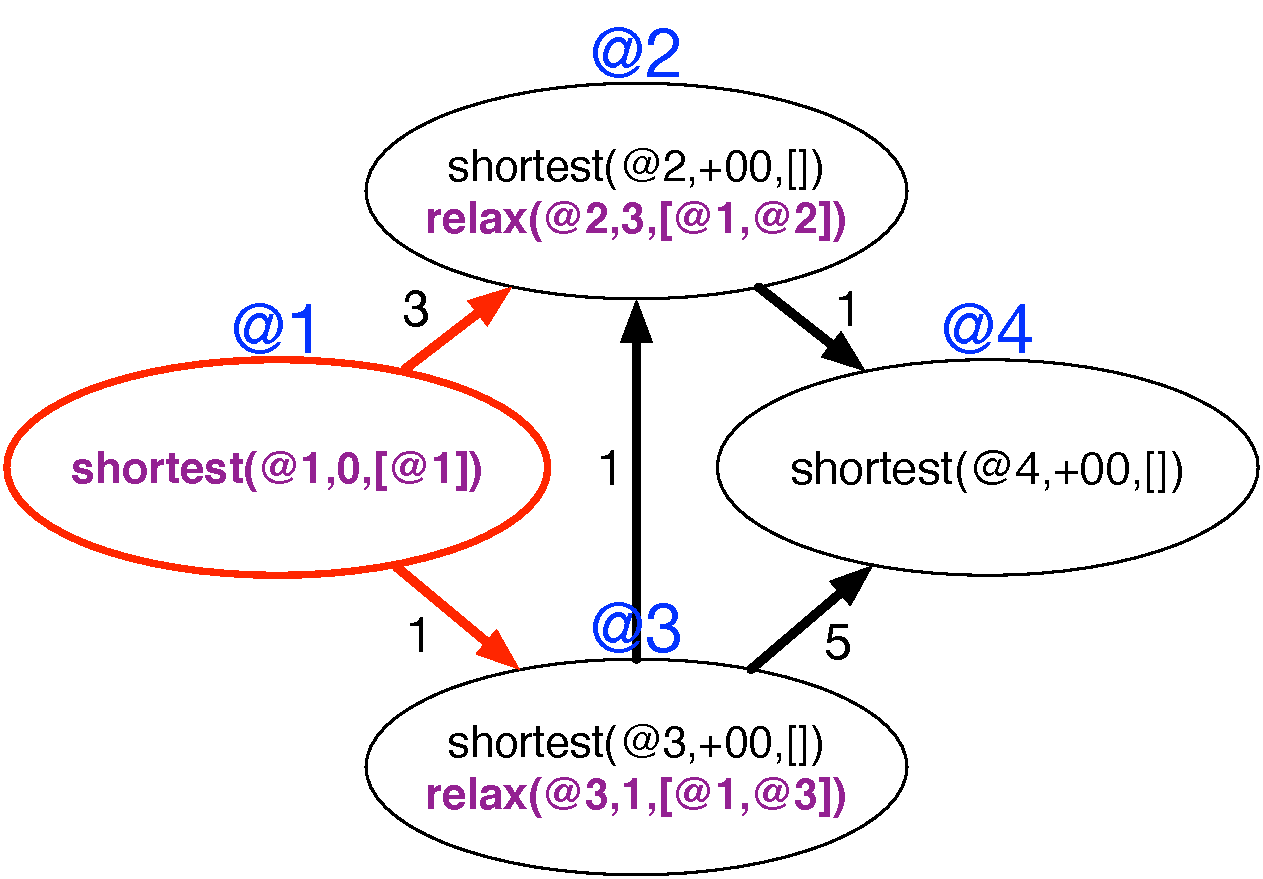
\includegraphics[width=\textwidth]{figures/sssp/coord1}
      \caption{}
   \end{subfigure}
   \begin{subfigure}[b]{0.49\textwidth}
      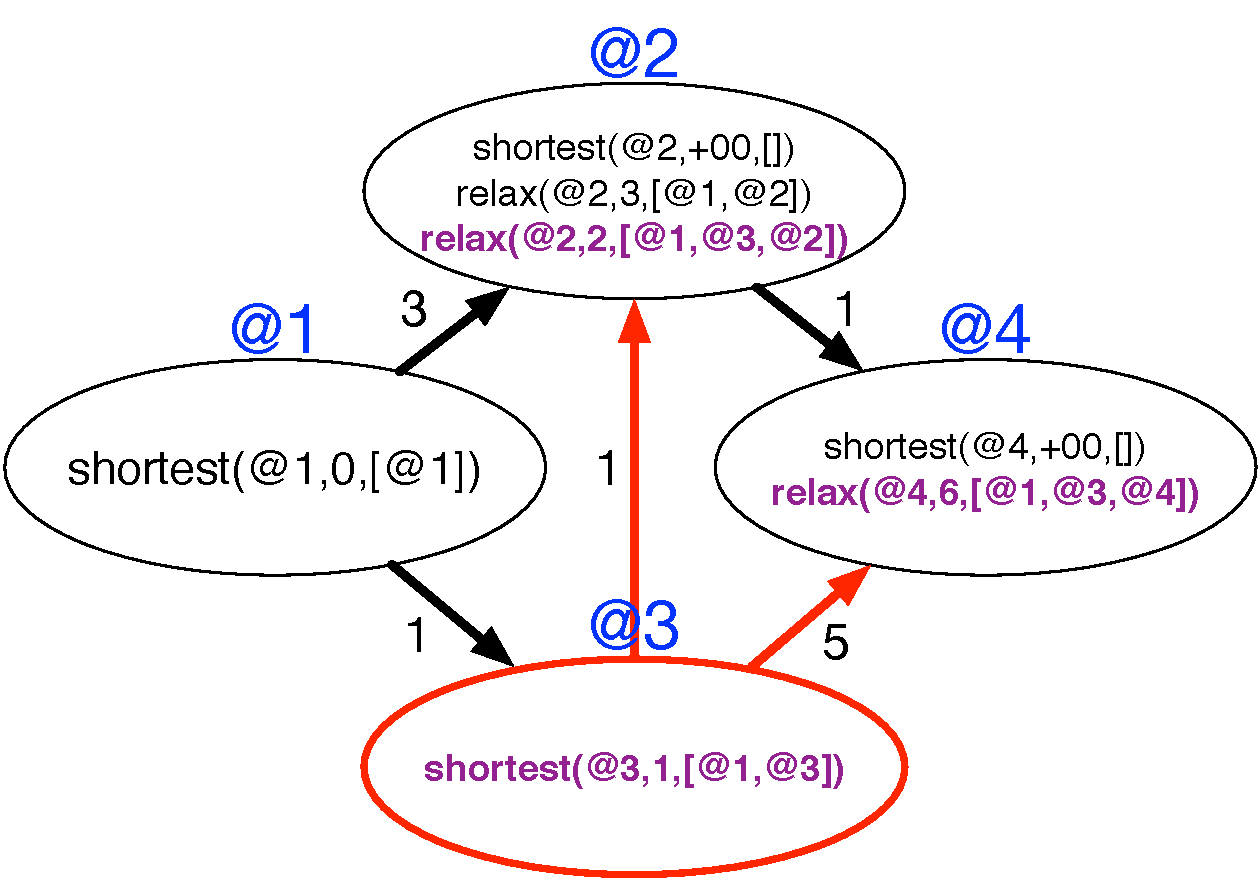
\includegraphics[width=\textwidth]{figures/sssp/coord2}
      \caption{}
   \end{subfigure}
   \begin{subfigure}[b]{0.49\textwidth}
      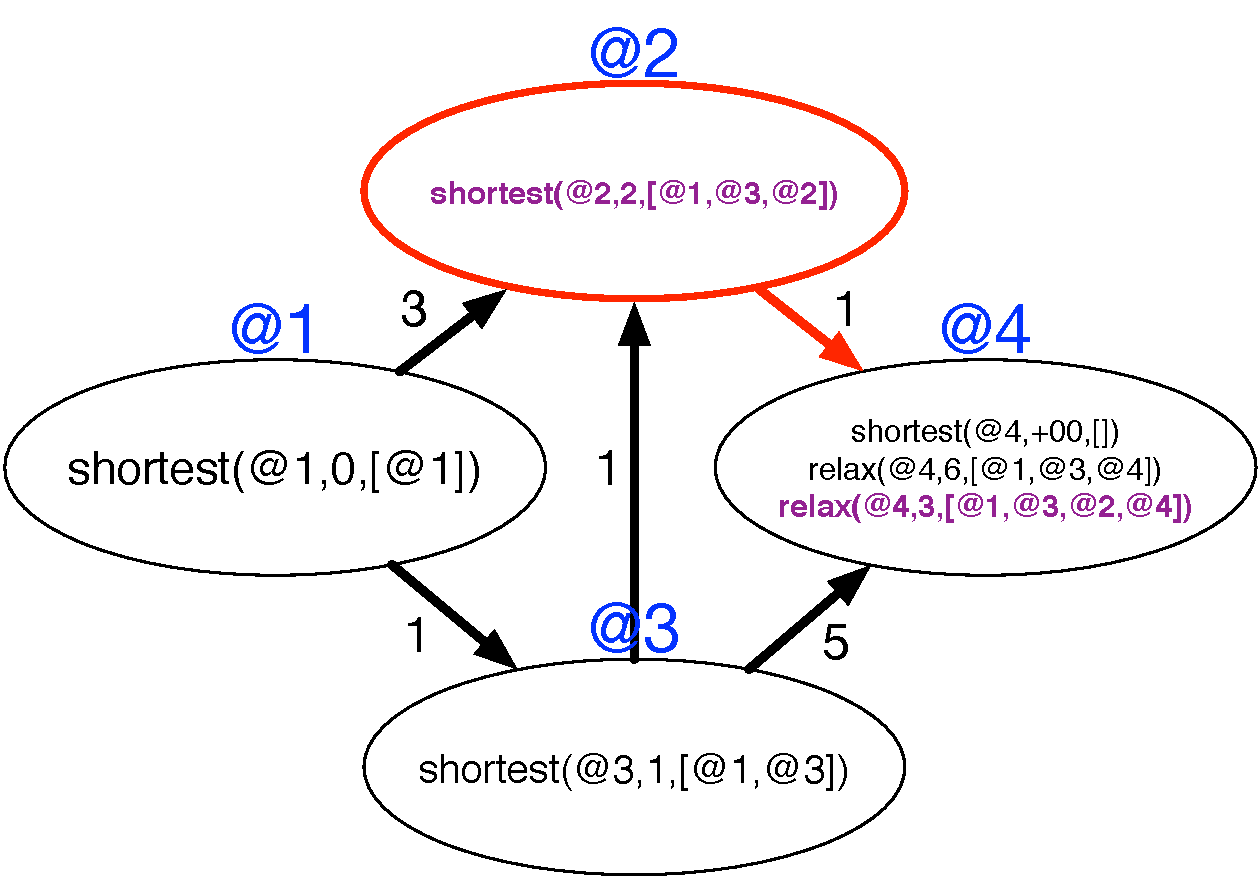
\includegraphics[width=\textwidth]{figures/sssp/coord3}
      \caption{}
   \end{subfigure}
   \begin{subfigure}[b]{0.49\textwidth}
      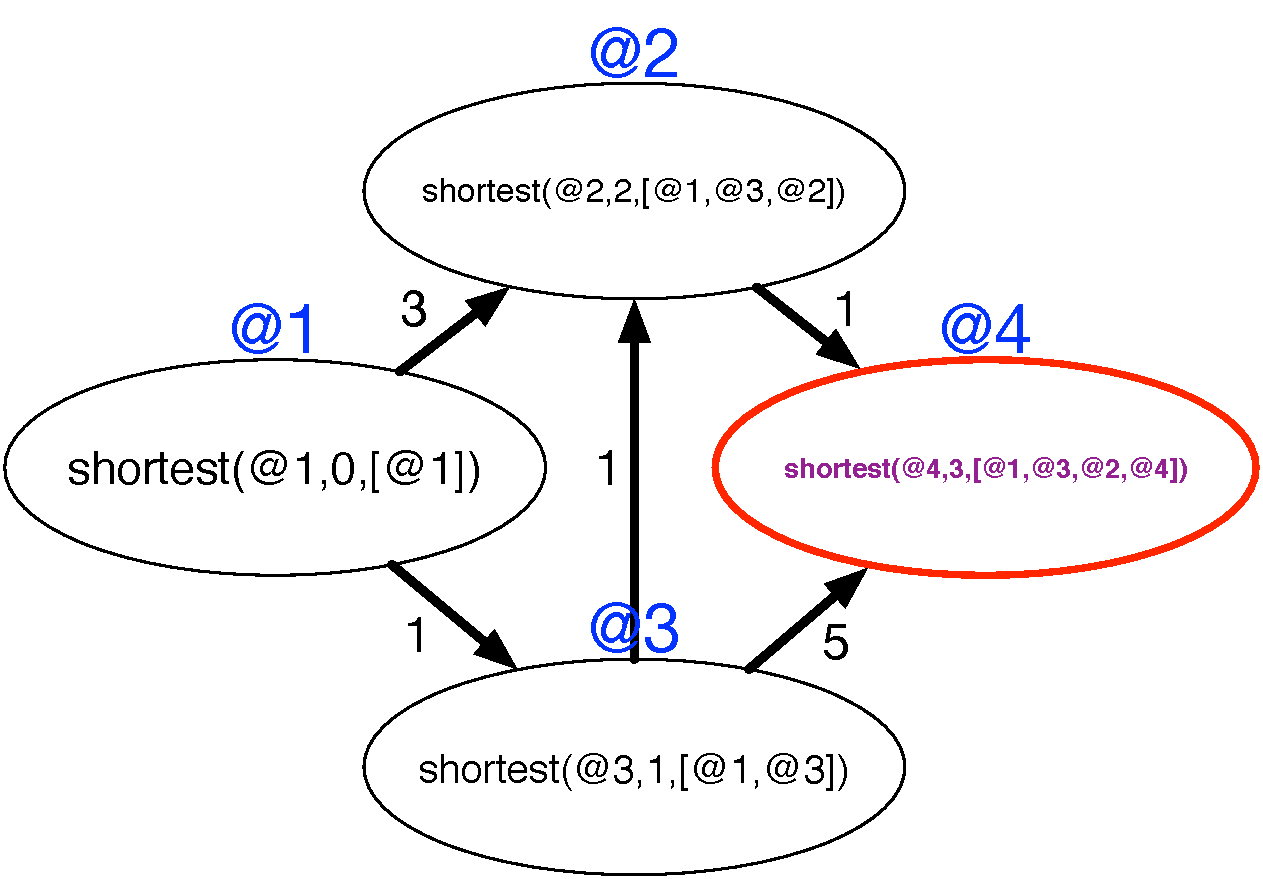
\includegraphics[width=\textwidth]{figures/sssp/coord4}
      \caption{}
   \end{subfigure}
\end{center}
\caption{Graphical representation of the new SSSP program in
   Fig.~\ref{code:shortest_path_program_coord}. (a) represents the
   program after propagating initial distance at node \code{@1}, followed by
   (b) where the first rule is applied in node \code{@3}. (c)
   represents the result after retracting all the \code{relax} facts at node
   \code{@2} and (d) is the final state of the program where all the shortest paths
   have been computed.}
\label{fig:coordination:new_sssp}
\end{figure}

In order to experiment with the coordinated SSSP program, we extend it to
support the computation of shortest distances from multiple sources. This
modified version, named MSSD was already used in
Section~\ref{section:implementation:performance} for measuring the performance
of LM's virtual machine. MSSD is not only more interesting than SSSP but also
allows us to better understand the advantages of using coordination.

Table~\ref{table:coordination:sssp_stats} presents fact statistics of the
regular and coordinated versions of MSSD when executed using 1 thread. We
gathered the number of facts derived, number of facts deleted, number of facts
sent (to other nodes) and the final number of facts. Note that the number of
facts sent is a subset of the number of facts derived, while the final number of
facts is the number of facts derived minus the number of facts deleted plus the
number of initial facts. As expected, there is a reduction in the number of
facts derived in all datasets. There is also a clear correlation between the
reduction in facts processed and the run time reduction achieved using
coordination.

\begin{table}[ht]
   \begin{center}
      \begin{tabular}{c | c || c | c | c | c} \hline
	\textbf{Program} & \textbf{Dataset} & \textbf{\# Derived} & \textbf{\# Sent} & \textbf{\# Deleted} & \textbf{\# Final} \\ \hline \hline
\multirow{7}{*}{Regular}  & US 500 Airports & 2.9M & 2.9M & 2.7M & 164.3K \\
 & OCLinks & 64.9M & 64.9M & 62.8M & 2.2M \\
 & EU Email & 35.4M & 34.9M & 32.7M & 3.8M \\
 & Twitter & 357.5M & 357.4M & 354.7M & 4.5M \\
 & US Power Grid & 207.6M & 207.6M & 183.2M & 24.4M \\
 & Live Journal & 731.8M & 721.4M & 723.9M & 71.5M \\
 & Orkut & 251.3M & 247.9M & 248.4M & 100.6M \\
	\hline
\multirow{7}{*}{Coordinated}  & US 500 Airports & 2.4M & 2.4M & 2.2M & 164.3K \\
 & OCLinks & 52.8M & 52.8M & 50.6M & 2.2M \\
 & EU Email & 24.1M & 23.6M & 20.2M & 3.8M \\
 & Twitter & 73.5M & 73.4M & 70.6M & 4.5M \\
 & US Power Grid & 135.5M & 135.5M & 111.1M & 24.4M \\
 & Live Journal & 134.7M & 128.9M & 126.8M & 71.5M \\
 & Orkut & 100.4M & 97.3M & 97.4M & 100.6M \\
	\hline
\end{tabular}

   \end{center}

   \caption{Fact statistics for the MSSD program when using 1 thread. For each
      dataset, we gathered the number of facts derived, number of facts deleted,
      number of facts sent to other nodes and total number of facts in the
      database when the program terminates.}

   \label{table:coordination:sssp_stats}
\end{table}

Figure~\ref{fig:coordination:results_sssp} shows the comparison between the
regular version (without coordination) and the coordinated version of the MSSD
program. We use the datasets already described in
Section~\ref{section:implementation:performance}.  In each plot we present the
following lines: \textbf{Regular}, which represents the run time of the regular
version; \textbf{Coordinated}, which represents the run time of the coordinated
version; \textbf{Regular(1)/Regular(t)}, which represents the speedup of the
regular version using the single threaded regular version as the baseline;
\textbf{Regular(1)/Coordinated(t)}, which represents the speedup of the
coordinated version against the run time of the regular version using 1 thread
as the baseline; and \textbf{C++}, which represents the run time of the MSSD C++
program already presented in Section~\ref{section:implementation:performance}.
Note that the run time (vertical axis) axis uses a logarithmic scale.

Overall, there is a clear improvement in almost every dataset used. The datasets
that see the best run time reductions are Twitter, Orkut and LiveJournal, which
are the datasets where the distance is calculated for less nodes. When
calculating the distance from multiple sources, the \code{set-priority} fact is
less effective because, although it selects the node with the shortest distance
to some source node, other distance computations (from other source nodes) are
also propagated to neighbor nodes, which may not be optimal. To solve this
particular issue, another kind of priority would have to be devised in order to
prioritize the computation of the shortest distance to only a single node.

\begin{figure}[]
        \centering
        \begin{subfigure}[b]{\plotsize\textwidth}
                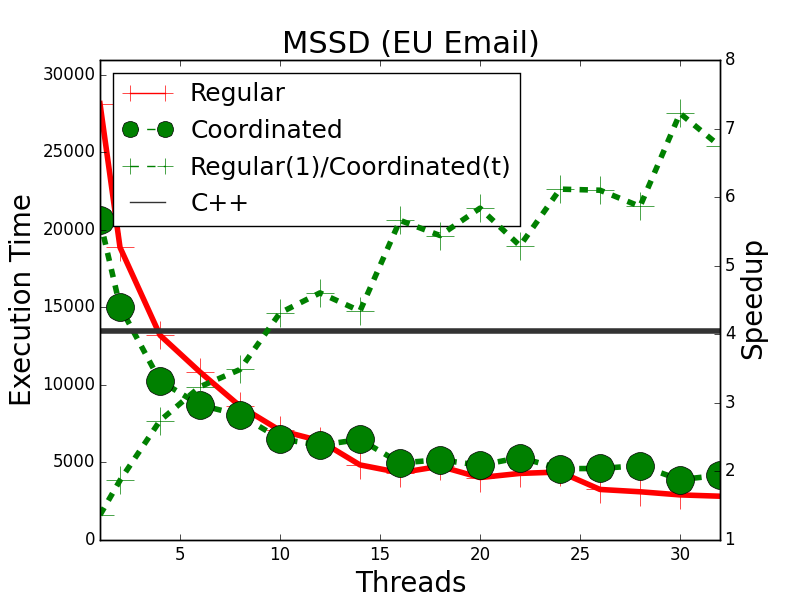
\includegraphics[width=\textwidth]{experiments/coordination/cmp-shortest-email.png}
                \label{fig:coordination:coord_sssp_email}
                \caption{Graph with 265000 nodes and 420000 edges. The shortest
                distance is calculated for 100 nodes.}
        \end{subfigure}
        ~
        \begin{subfigure}[b]{\plotsize\textwidth}
                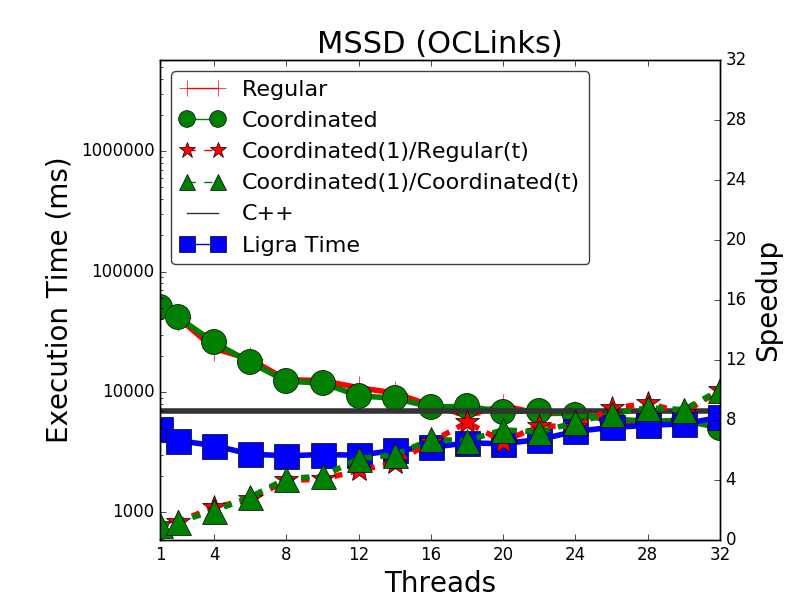
\includegraphics[width=\textwidth]{experiments/coordination/cmp-shortest-oclinks.png}
                \label{fig:coordination:coord_sssp_oclinks}
                \caption{Graph with around 2000 nodes and 20000 edges. The shortest
                   distance is calculated for all nodes.}
        \end{subfigure} \\
        \begin{subfigure}[b]{\plotsize\textwidth}
                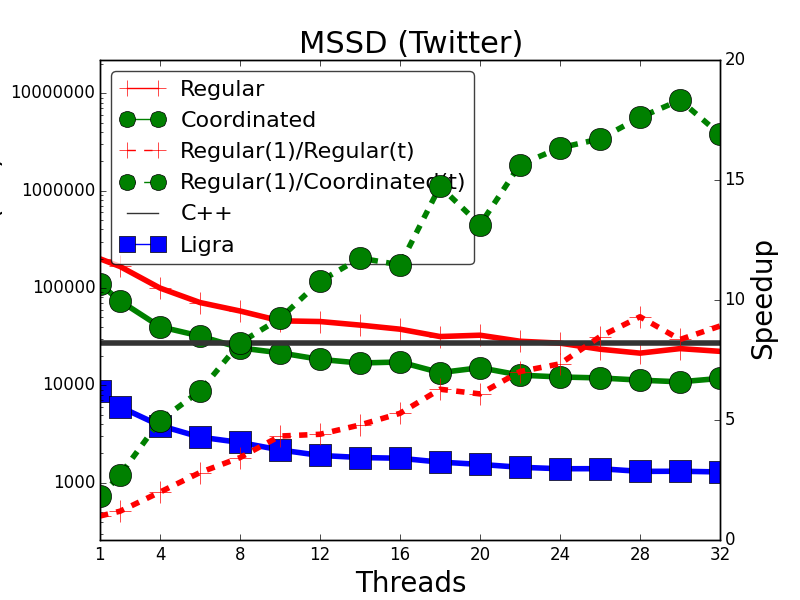
\includegraphics[width=\textwidth]{experiments/coordination/cmp-shortest-twitter.png}
                \label{fig:coordination:coord_sssp_twitter}
                \caption{Graph with 81306 nodes and 1768149 edges. The shortest
                   distance is calculuated for 40 nodes.}
        \end{subfigure}
        ~
        \begin{subfigure}[b]{\plotsize\textwidth}
                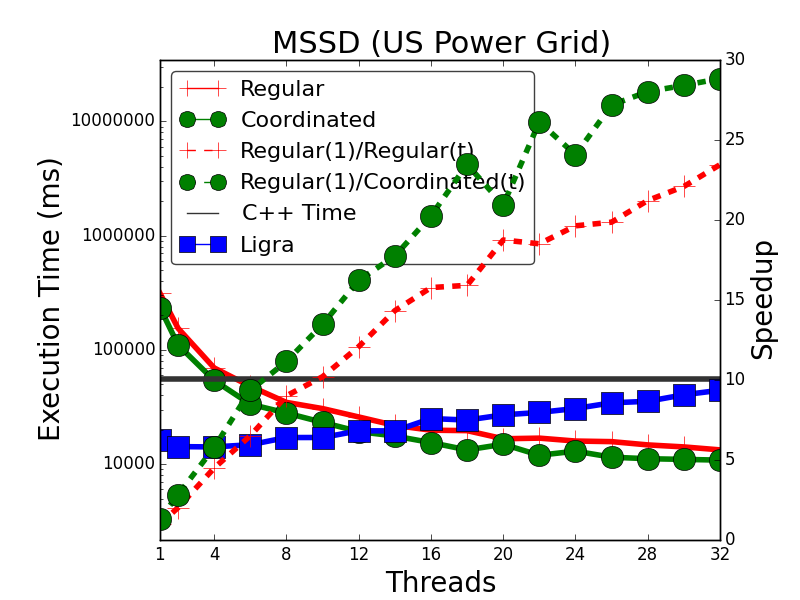
\includegraphics[width=\textwidth]{experiments/coordination/cmp-shortest-uspowergrid.png}
                \label{fig:coordination:coord_sssp_uspowergrid}
                \caption{Graph with around 5000 nodes and 13000 edges. The
                shortest distance is calculated for all nodes.}
        \end{subfigure}\\
        \begin{subfigure}[b]{\plotsize\textwidth}
                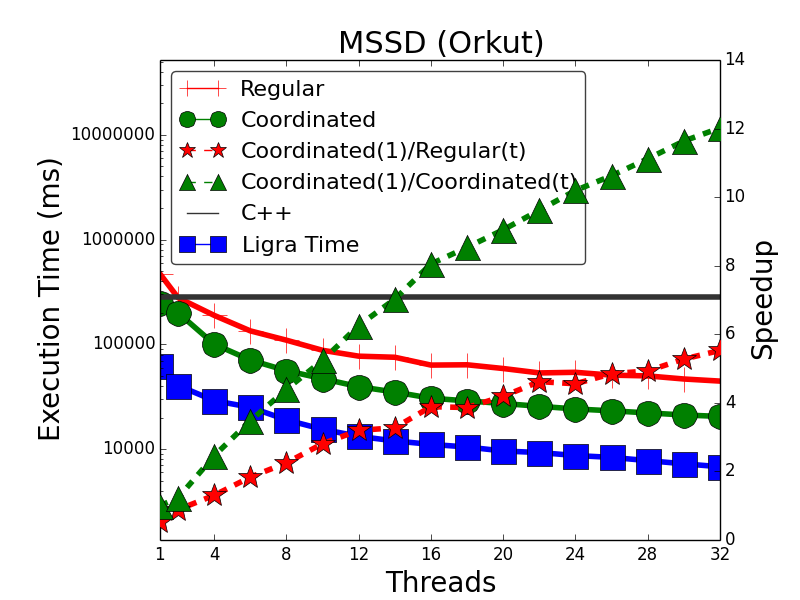
\includegraphics[width=\textwidth]{experiments/coordination/cmp-shortest-orkut.png}
                \label{fig:coordination:coord_sssp_orkut}
                \caption{Graph with 3072441 nodes and 117185083 edges. The shortest
                   distance is calculated for two nodes.}
        \end{subfigure}
        ~
        \begin{subfigure}[b]{\plotsize\textwidth}
                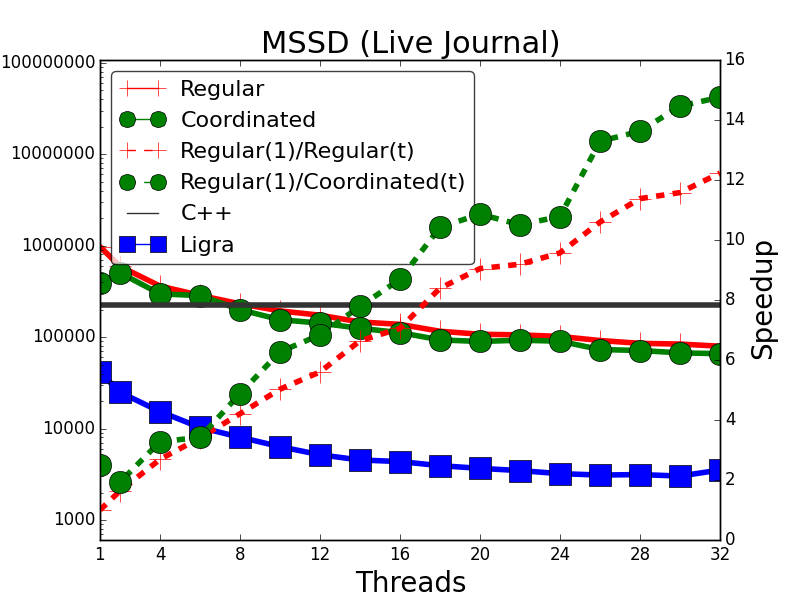
\includegraphics[width=\textwidth]{experiments/coordination/cmp-shortest-livejournal.png}
                \label{fig:coordination:coord_sssp_livejournal}
                \caption{Graph with around 4847571 nodes and 68993773 edges. The
                shortest distance is calculated for two nodes.}
        \end{subfigure}\\

        \caption{Scalability comparison for the MSSD program when enabling
        coordination facts.}

        \label{fig:coordination:results_sssp}
\end{figure}

There is another interesting trend in our results which relates the improvement
offered by the coordination version over the regular version and the number of
threads used. Even if the number of threads goes up, the coordinated version is
still able to keep about the same run time reduction ratio over the regular
version. This means that even if higher priority nodes are picked from the each
thread's subgraph, the coordinated version is still able to reduce run time. In
other words, optimal (global) node scheduling is not required to see good
results.

In Section~\ref{section:coordination:coord_instrs}, we described the coalescing
optimization where priority action facts are coalesced into single operations.
The MSSD program computes shortest distances to multiple nodes and thus it can
take advantage of this optimization. Consider a MSSD program that is computing
the shortest distances from node \code{@1} and \code{@2}. If a node \code{@3}
needs to propagate the shortest distance $d_1$ to another node \code{@4}
(distance from \code{@1}) and a distance $d_2$ to node \code{@4} (distance from
\code{@2}), then it would need to change the priority twice, first to $d_1$, and
then to $d_2$.  With the coalescing optimization, it only changes the priority
to the best of both.  It is then advantageous to only apply a single
coordination operation in order to reduce queue operations and overall locking.

In order to observe the effects of the coalescing optimization, we disabled its
support from the VM and then we ran the same experiments where priority updates
are done immediatelly. The results are presented in
Fig.~\ref{fig:coordination:results_sssp_unbuffered}. From the results, we can
see that some datasets, such as EU Email and US Power Grid, maintain their
overall scalability, especially the speedup (\textbf{Regular(1)/Coordinated(t)})
for 32 threads (\textbf{t = 32}). For the OCLinks and Twitter datasets, there is
some performance degradation since their overall scalability drops without the
optimization. However, the Live Journal dataset improves its performance and
scalability when the optimization is disabled, since we only compute the
shortest distance for 2 nodes, therefore the opportunities for optimization are
fewer and supporting it ends up slowing the program. Interestingly, the same
does not happen for the Orkut dataset because the number of edges is much higher
and disabling the optimization makes the program perform slightly worse.  For
all the other datasets, we compute the shortest distance from an appreciable
number of nodes and the coalescing optimization is worth its cost.


\begin{figure}[]
        \centering
        \begin{subfigure}[b]{\plotsize\textwidth}
                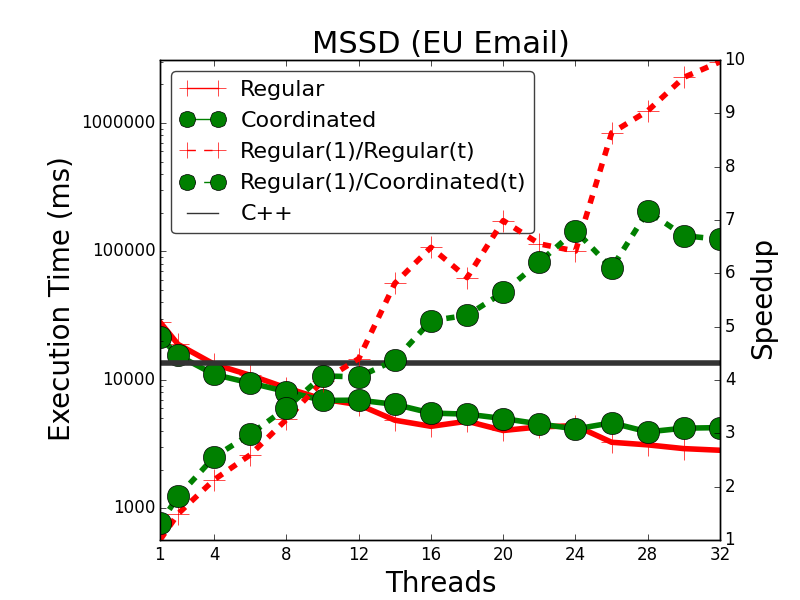
\includegraphics[width=\textwidth]{experiments/coordination/unbuffered-shortest-email.png}
                \label{fig:coordination:coord_unbuffered_sssp_email}
                \caption{Graph with 265000 nodes and 420000 edges. The shortest
                distance is calculated for 100 nodes.}
        \end{subfigure}
        ~
        \begin{subfigure}[b]{\plotsize\textwidth}
                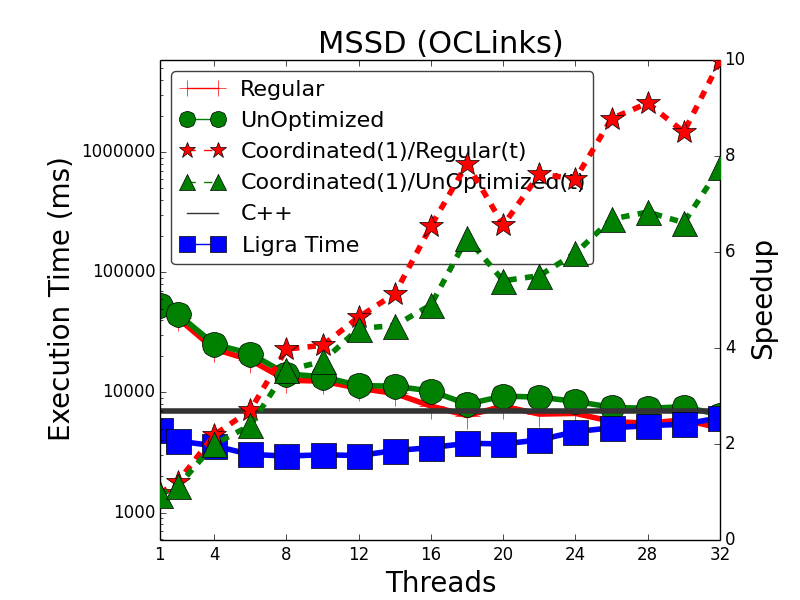
\includegraphics[width=\textwidth]{experiments/coordination/unbuffered-shortest-oclinks.png}
                \label{fig:coordination:coord_unbuffered_sssp_oclinks}
                \caption{Graph with around 2000 nodes and 20000 edges. The shortest
                   distance is calculated for all nodes.}
        \end{subfigure} \\
        \begin{subfigure}[b]{\plotsize\textwidth}
                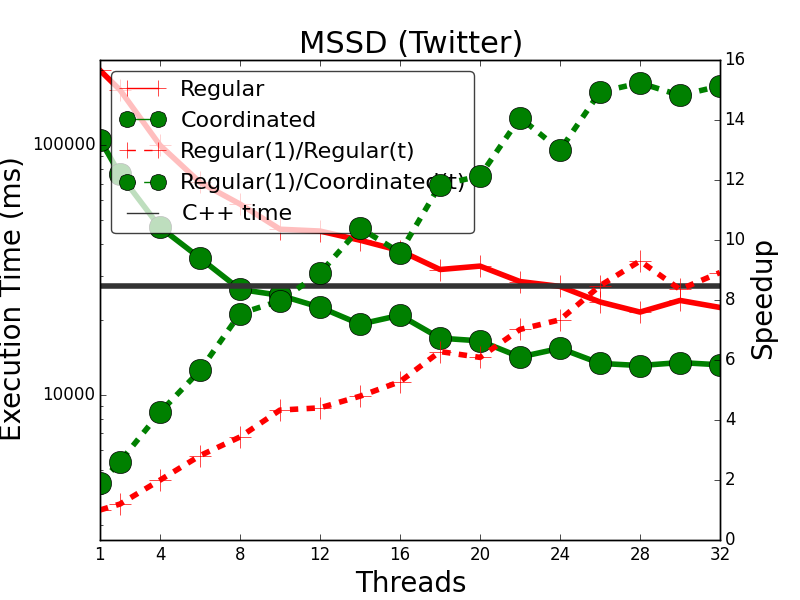
\includegraphics[width=\textwidth]{experiments/coordination/unbuffered-shortest-twitter.png}
                \label{fig:coordination:coord_unbuffered_sssp_twitter}
                \caption{Graph with 81306 nodes and 1768149 edges. The shortest
                   distance is calculuated for 40 nodes.}
        \end{subfigure}
        ~
        \begin{subfigure}[b]{\plotsize\textwidth}
                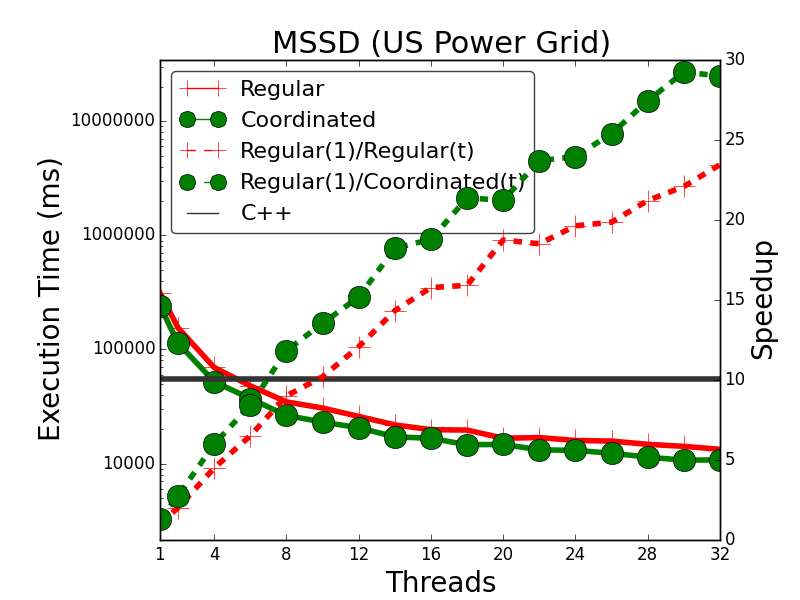
\includegraphics[width=\textwidth]{experiments/coordination/unbuffered-shortest-uspowergrid.png}
                \label{fig:coordination:coord_unbuffered_sssp_uspowergrid}
                \caption{Graph with around 5000 nodes and 13000 edges. The
                shortest distance is calculated for all nodes.}
        \end{subfigure}\\
        \begin{subfigure}[b]{\plotsize\textwidth}
                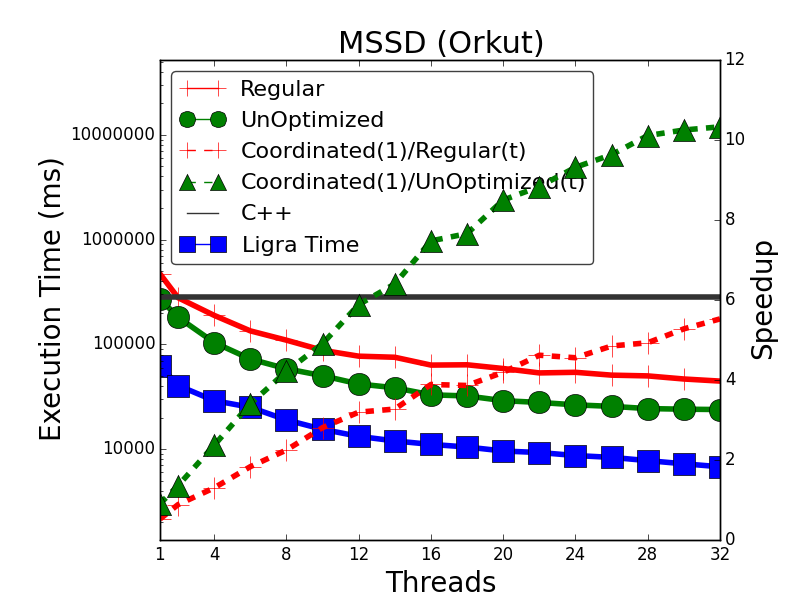
\includegraphics[width=\textwidth]{experiments/coordination/unbuffered-shortest-orkut.png}
                \label{fig:coordination:coord_unbuffered_sssp_orkut}
                \caption{Graph with 3072441 nodes and 117185083 edges. The shortest
                   distance is calculated for two nodes.}
        \end{subfigure}
        ~
        \begin{subfigure}[b]{\plotsize\textwidth}
                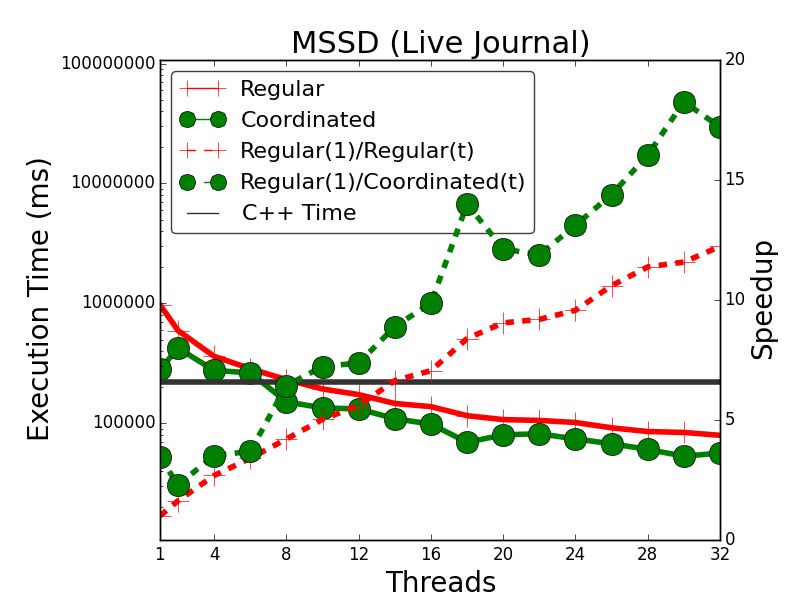
\includegraphics[width=\textwidth]{experiments/coordination/unbuffered-shortest-livejournal.png}
                \label{fig:coordination:coord_unbuffered_sssp_livejournal}
                \caption{Graph with around 4847571 nodes and 68993773 edges. The
                shortest distance is calculated for two nodes.}
        \end{subfigure}\\

        \caption{Scalability for the MSSD program when not coalescing
        coordination directives.}

        \label{fig:coordination:results_sssp_unbuffered}
\end{figure}


